\newpage
\subsection*{Double Side Band -- Suppressed Carrier (DSB-SC)}
\addcontentsline{toc}{subsection}{DSB-SC}
The DSB-SC signal is implemented using a balanced modulation technique, where the message
signal is directly multiplied with the carrier signal. This multiplication suppresses the
carrier component while producing both upper and lower sidebands. In the implementation,
time-domain plots are used to visualize the modulated waveform, and frequency-domain
analysis is carried out to verify the absence of the carrier and the presence of symmetric
sidebands around the carrier frequency.

\subsubsection*{Code:}

\begin{minted}[linenos, fontsize=\small]{python}
import numpy as np
import matplotlib.pyplot as plt

# Sampling Parameters
Fs = 10000                 # Sampling frequency (Hz)
T = 0.1                   # Duration of signal (seconds)
t = np.arange(0, T, 1/Fs)  # Time vector

# Baseband signal (message)
Am = 1                     # Message amplitude
fm = 50                    # Message frequency (Hz)
m_t = Am * np.sin(2 * np.pi * fm * t)

# Carrier signal
fc = 1000                         # Carrier frequency (Hz)
c_t = np.cos(2 * np.pi * fc * t)  # amplitude = 1 for DSB-SC

# DSB-SC Modulated signal
s_dsbsc = m_t * c_t  # No carrier term added

# Time-domain plots
plt.figure(figsize=(12, 8))

plt.subplot(3,1,1)
plt.plot(t, m_t, 'b', linewidth=1.5)
plt.title('Message Signal m(t)')
plt.xlabel('Time [s]')
plt.ylabel('Amplitude')
plt.xlim(0, 0.05)
plt.grid(True)

plt.subplot(3,1,2)
plt.plot(t, c_t, 'r', linewidth=1.5)
plt.title('Carrier Signal c(t)')
plt.xlabel('Time [s]')
plt.ylabel('Amplitude')
plt.xlim(0, 0.05)
plt.grid(True)

plt.subplot(3,1,3)
plt.plot(t, s_dsbsc, 'g', linewidth=1.5)
plt.title('DSB-SC Modulated Signal s(t)')
plt.xlabel('Time [s]')
plt.ylabel('Amplitude')
plt.xlim(0, 0.05)
plt.grid(True)

plt.tight_layout()
plt.show()

# Frequency-domain analysis
N = len(s_dsbsc)
S_f = np.fft.fft(s_dsbsc)/N
f = np.fft.fftfreq(N, 1/Fs)

f_pos = f[:N//2]
S_f_pos = 2 * np.abs(S_f[:N//2])

plt.figure(figsize=(10,4))
plt.plot(f_pos, S_f_pos, 'm', linewidth=1.5)
plt.title("Magnitude Spectrum of DSB-SC Signal")
plt.xlabel("Frequency [Hz]")
plt.ylabel("Magnitude")
plt.grid(True)
plt.xlim(fc - 200, fc + 200)
plt.show()
\end{minted}

\subsubsection*{Output:}
The above plots are obtained using the following parameters: sampling frequency
$F_s = 10~\text{kHz}$, signal duration $T = 0.1~\text{s}$, message amplitude
$A_m = 1$, carrier amplitude $A_c = 1$, message frequency $f_m = 50~\text{Hz}$,
and carrier frequency $f_c = 1000~\text{Hz}$.

\begin{figure}[h!]
    \centering
    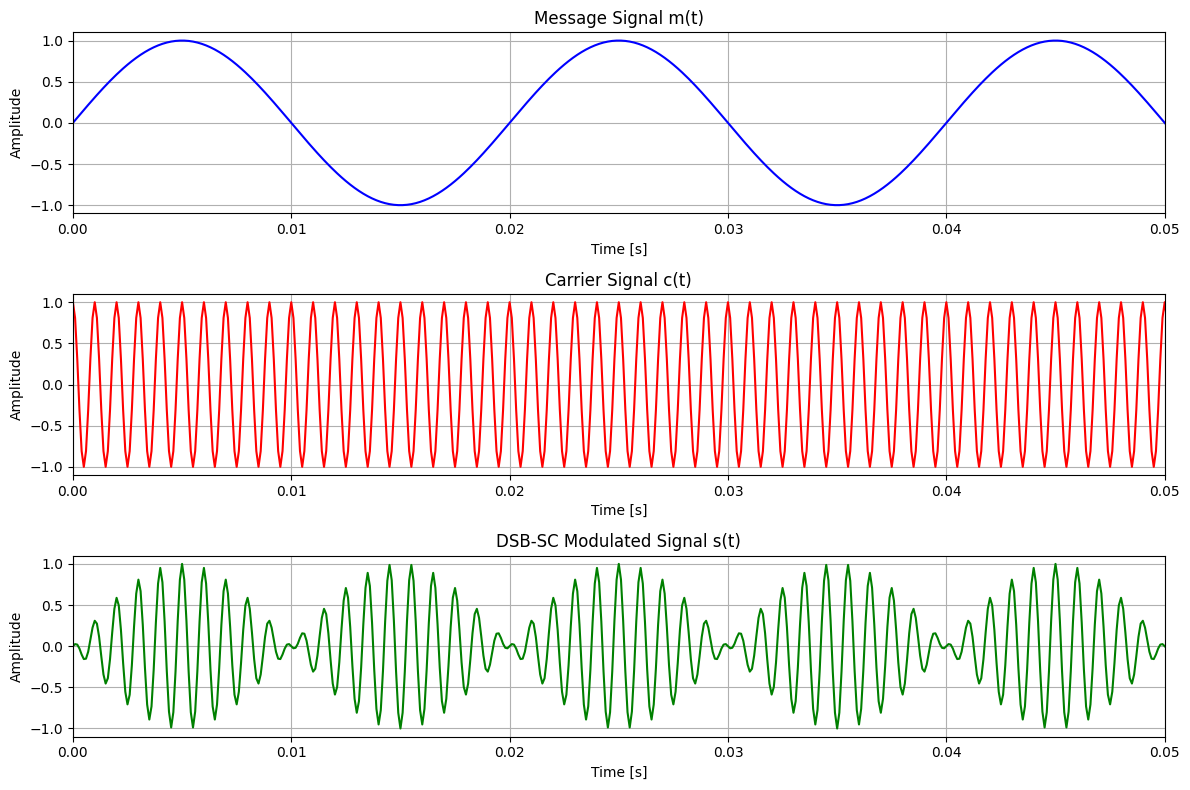
\includegraphics[width=0.9\textwidth]{images/output3.png} 
    \caption{Plots of (a) Message Signal, (b) Carrier Signal, and (c) DSB-SC Modulated Signal}
    \label{fig:output3}
\end{figure}
\begin{figure}[h!]
    \centering
    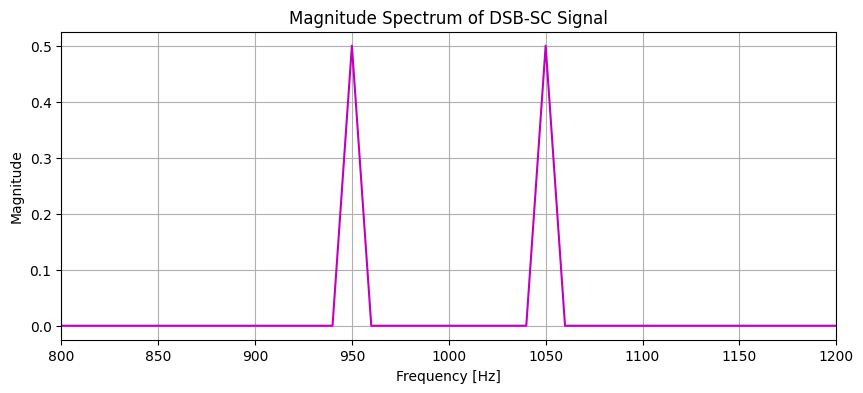
\includegraphics[width=0.9\textwidth]{images/output4.png} 
    \caption{Plots of DSB-SC spectrum (0.1s)}
    \label{fig:output4}
\end{figure}
\begin{figure}[h!]
    \centering
    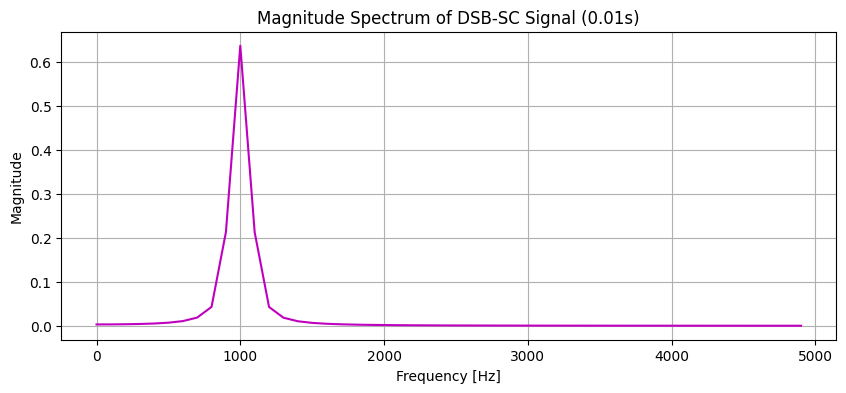
\includegraphics[width=0.9\textwidth]{images/output5.png} 
    \caption{Plots of DSB-SC spectrum (0.01s)}
    \label{fig:output5}
\end{figure}


\subsubsection*{Observations:}

Although DSB-SC modulation theoretically suppresses the carrier completely, a small
spectral component near the carrier frequency is observed in the FFT when the signal
duration is reduced to $T = 0.01~\text{s}$. This occurs due to limited frequency
resolution and spectral leakage associated with finite-duration signals. Increasing
the signal duration improves the frequency resolution of the FFT, thereby reducing
this effect and clearly revealing only the upper and lower sidebands.